The CLiCs database is available online at \url{http://lingulist.de/clics/} and offers its users a search interface to all concepts and cross-linguistic colexifications between concepts. The wealth of information in the database and the various possibilities of exploring the colexifications in the network call for an additional component that makes potentially interesting observations more easily accessible to the researcher. The idea was to equip the database with a visualization component that provides various interactive functionalities and enables users to navigate through the networks of colexifications while at the same time providing more detailed information on the actual language data. A prototype of the visualization is online accessible.\footnote{\url{http://tinyurl.com/clicsvis}}

\subsection{Web-based visualization}
% why web-based? main advantages

We opted for a web-based implementation of the CLiCs visualization in JavaScript using the D3 library \cite{D3}. The main benefits of a web-based visualization are its platform independence and the fact that users can access it from any device with a browser supporting JavaScript. There is no need for the installation of additional software or for maintenance of the system on the part of the user \cite{Murray}. In addition, links to the descriptions of the external resources can easily be included to allow users to explore the CLiCs data in more detail on demand. 

\subsection{Data Preparation}
In its current form, the data in CLiCs yields a \emph{small world network} in which all nodes are
densely connected. Browsing such a full network is very confusing and provides little insights for
the user (see Figure \ref{fig:clics_full}). In order to break down the complexity inherent in CLiCs,
we decided to split the data into communities first.  Starting from 1285 concepts in CLiCs which
were connected to at least one other concept, we applied the \emph{Infomap} algorithm by
\newcite{Rosvall2008} to cluster all concepts into communities, using the number of attested
language families per colexification as edge weights. The Infomap algorithm was chosen because of
its remarkable performance on the community detection task, both in terms of computation time and
quality of results \cite{Lancichinetti2009}.
With help of this analysis, the 1285 concepts
could be subdivided into 160 communities of which 156 contain more than one node. 
Of all communities, 106 are \emph{large}, containing more than
five nodes. The large communities cover 88\% (1125) of all nodes in the original network (1285). In
order to enable the user to quickly identify communities of specific interest, we labelled all
communities by taking the concept with the highest degree as a representative. Apart from one very
large community of 102 concepts (``do, make"), the rest of the communities does not differ much in
size, ranging from 2 (``meeting house") to 26 concepts (``get, obtain") with an average of 8 concepts per community.

\begin{figure}[b]
    \centering
   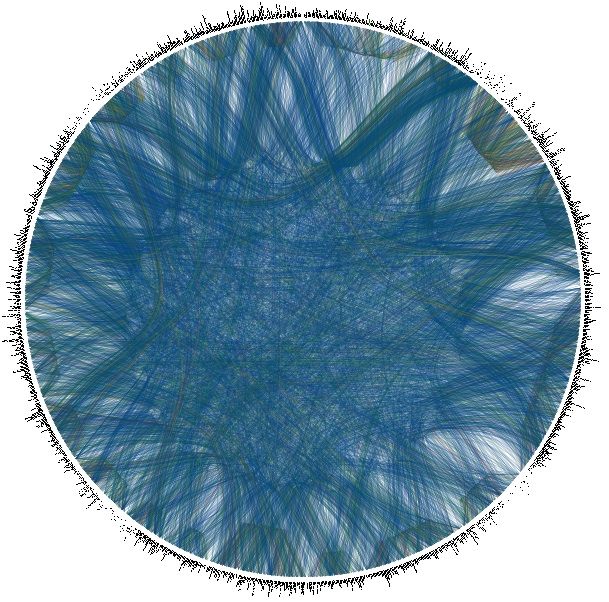
\includegraphics[width=0.48\textwidth]{img/completeNetworkLabels.jpg}
    \caption{Full network of all 1285 concepts in CLiCs (outer circle) together with their connections. The strength of the connections is marked in different colors, with very strong links represented in red}
    \label{fig:clics_full}
\end{figure}
\subsection{Interactive functionalities}


% Force-directed graph; move nodes to desired position

The visualization features various interactive functionalities that are designed to enhance the exploration of the CLiCs data on the level of communities. The main component is a flexible force-directed graph layout that displays the concepts as nodes and the cross-linguistic polysemies as edges (see Figure \ref{EarthLand}). The strength of the force in the edges of the graph is dependent on the number of cases that can be attested in the languages for the respective concepts that are linked through the edge. We decided to have separate graphs for all communities, which the user can select from a drop-down menu. As described above, the communities have been automatically generated from the whole network of concepts and links with the help of the Infomap algorithm for community detection \cite{Rosvall2008}. 

\begin{figure}[htbp]
\begin{center}
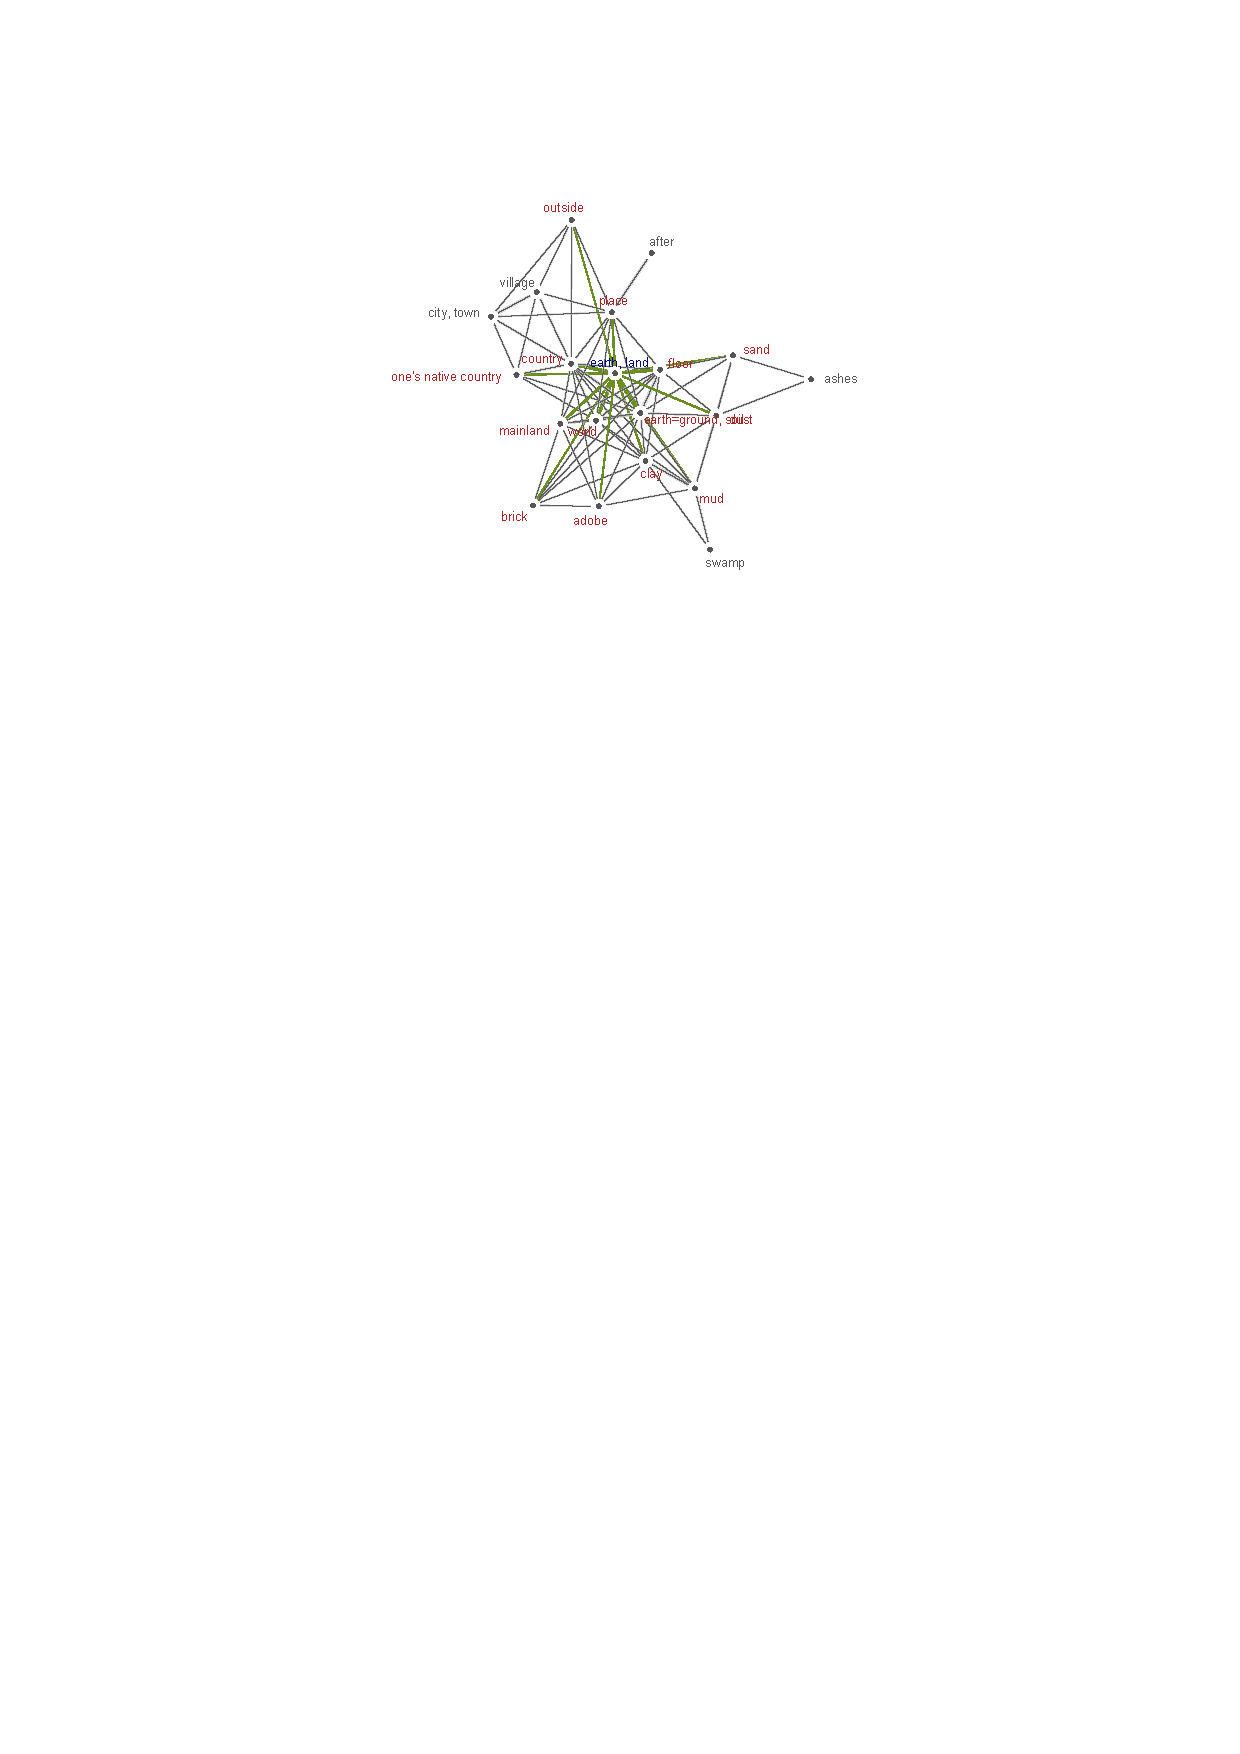
\includegraphics[width=0.48\textwidth]{img/countryconnections}
\caption{Force-directed graph with mouse-over functionalities highlighting all connected concepts}
\label{EarthLand}
\end{center}
\end{figure}

The force-directed graph layout ensures that all concepts are neatly arranged according to their similarity as defined by the number of cross-linguistic colexifications. As a result, concepts that are highly connected are located close to each other.  To make it easier for users to explore the network that is depicted in the graph, concepts can be dragged to different positions where there is less overlap. The dragging behavior of a concept  is activated when mousing over the respective node in the graph (when the cursor symbol turns into a crosshair).

\begin{figure*}[htbp]
\begin{center}
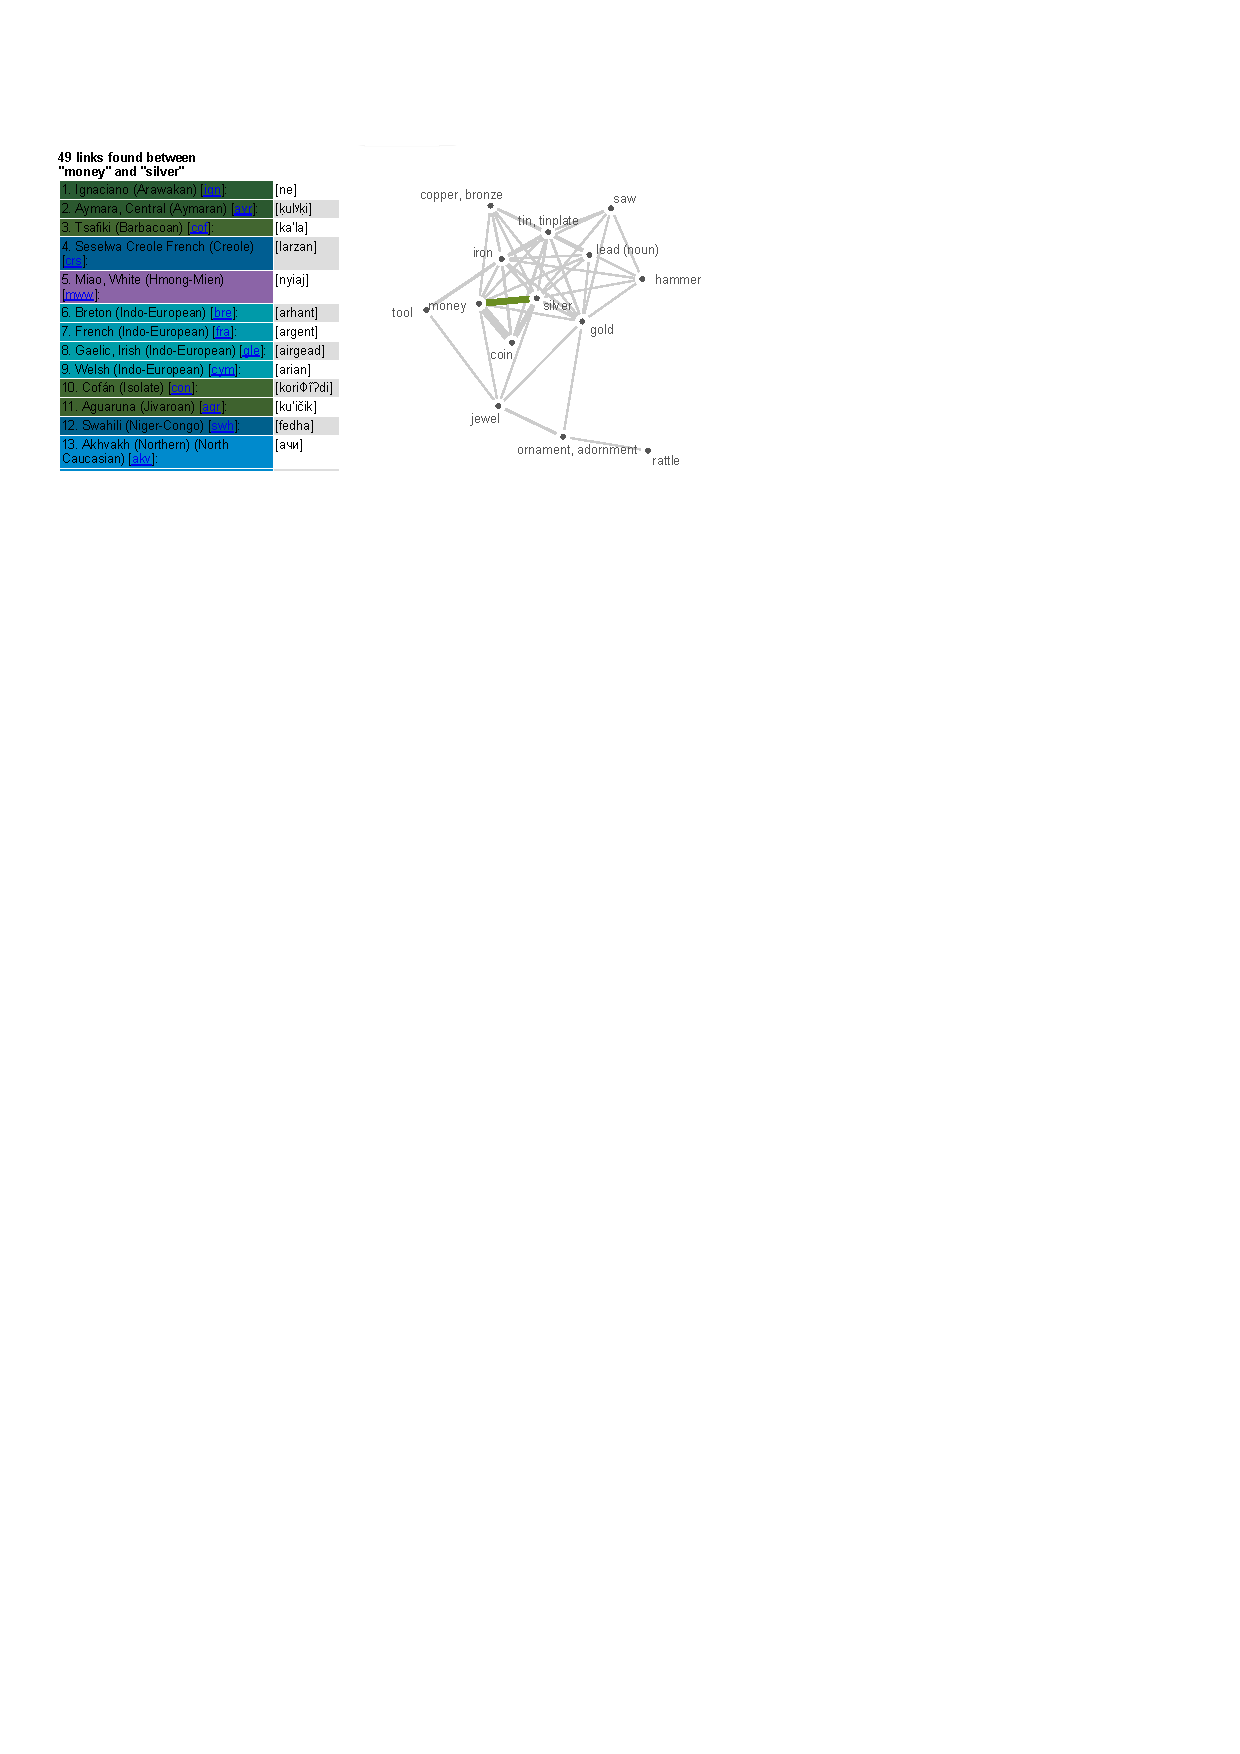
\includegraphics[width=\textwidth]{img/moneysilverexample.pdf}
\caption{Force-directed graph with mouse-over functionalities showing a subset of the list of words contributing to the cross-linguistic polysemies. The entries have different background colors depending on their location in the world map (cf. Figure \ref{World map}).}
\label{MoneySilver}
\end{center}
\end{figure*}



% mouse-over: coloring edges, show linked languages

As mentioned above, the edges of the graph represent the number of cases of cross-linguistic colexifications for the linked concepts. For a more detailed view on which languages contribute to the strength of the connections, the user can mouse over the links in the graph to see a list of  languages featuring polysemous words for the respective link (Figure \ref{MoneySilver}). The list includes additional information on the languages such as their ISO 639-3 language code and family. Furthermore, each entry in the list provides a hyperlink to the original source from where the information is taken.  

% Color coding: families and geolocations

Each language in the list is attributed a different background color depending on its language family or location in order to allow for an at-a-glance overview for all languages in the list. The user can choose from a drop-down menu whether to include the genealogical or areal information as the background color. For the genealogical information, all language families are attributed a different color value. Languages belonging to the same language families are therefore given the same background color. Moreover, the list is sorted according to language families. In this way, the user can immediately see how many languages of  a given family contribute to the overall strength for the connection at hand. 

As to the areal information, the world map is provided with a color gradient as shown in Figure \ref{World map}. To this end, each position in the world map is attributed a color value using the L*a*b* color space. The color hue thereby indicates the position on the map in terms of the longitude (East-West) whereas the lightness of the color represents the position in terms of the latitude information (North-South).\footnote{See \cite{MayerLanguageExplorer} for a different approach of a linguistically informed color gradient of the world map.}
The mapping from geolocation to color values allows for an easier evaluation of areal patterns in the selected connection. In this regard, users can directly detect whether a certain cross-linguistic polysemy is restricted to a certain region of the world or constitutes a more widespread colexification pattern (see the case study in Section \ref{case study} below).

\begin{figure}[htbp]
\begin{center}
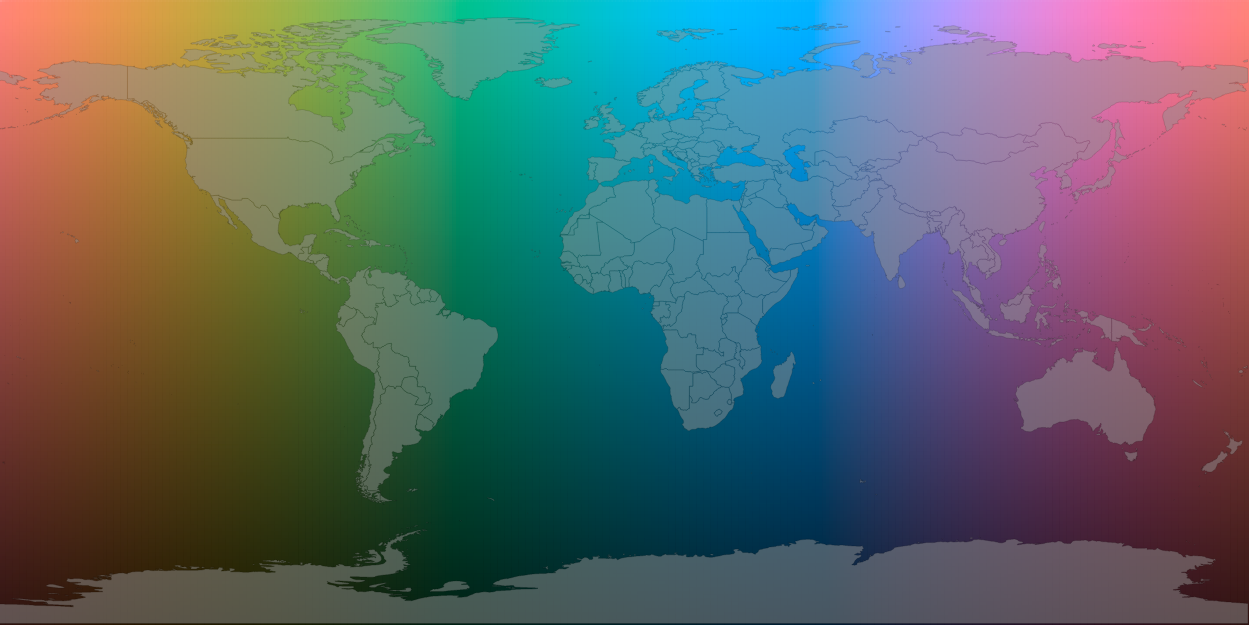
\includegraphics[width=0.48\textwidth]{img/ColorScaleWorld.png}
\caption{World map with color gradient}
\label{World map}
\end{center}
\end{figure}


% show only edges with a minimum number of links

In addition to the interactive functionalities described above, the visualization also features a variety of further components that allow for an easier exploration of the database. The graph layout is equipped with panning and zooming functionality that enables the user to navigate through the network graph. Panning is enabled when the cursor changes into a hand symbol when mousing over a link of the graph. The whole graph can then be dragged to a new position. The zooming behavior is activated with the scroll wheel. 
When mousing over a concept (node) in the graph all connected links and concepts are highlighted
in order to provide a better overview of the connectivity of certain concepts (see Figure \ref{EarthLand}). The control panel of the visualization also includes a slider button that allows the user to show only those edges in the graph with a minimum number of cross-linguistic colexifications. 

% zooming and panning



\subsection{Implementation}
% description of D3 and the implementation

The visualization is implemented in JavaScript using the D3 library \cite{D3}.\footnote{\url{http://d3js.org}} The force-directed graph is  generated with the \texttt{force()} function from the \texttt{d3.layout} module. The layout implementation uses position Verlet integration for simple constraints \cite{Dwyer2009}.\footnote{See \url{https://github.com/mbostock/d3/wiki/Force-Layout} for a description of the implementation.} In order to ensure that the concept labels are located close to the concept nodes, a second force layout (with a static weight of $1$) for each concept link to the node is set up. 

The color values for the world map gradient scale are computed from the two-dimensional geographical coordinates that are given as an input. The latitude [-90;90] and longitude [-180;180] values are thereby normalized between [0;1] and serve as the input for the function \texttt{cl2pix}.\footnote{The code was adapted from the GNU C code by David Dalrymple (\url{http://davidad.net/colorviz/}) and translated into JavaScript.}

\begin{verbatim}
function cl2pix(c,l){
   		var TAU = 6.2831853 
   		var L = l*0.61 + 0.09; 
   		var angle = TAU/6.0 - c*TAU;   
   		var r = l*0.311 + 0.125 
   		var a = Math.sin(angle)*r;
   		var b = Math.cos(angle)*r;
   		return [L,a,b];
 };
\end{verbatim}

The actual HTML color code is generated with the function \texttt{d3.lab} from the D3 library, which takes as input the three values for \texttt{[L,a,b]}. The main reason for choosing the L*a*b* color space is a smoother transition between different color hues without any visible boundaries.\footnote{See \url{http://davidad.net/colorviz/} for the difference between using the L*a*b* and HSV color space in terms of transitions between different color hues.} For the coloring of the language families, the background colors are generated with the categorical scale functions of the \texttt{d3.scale} module. 


The  dragging and panning functionalities of the graph are implemented with the \texttt{drag()} function from the \texttt{d3.behavior} module and the SVG \texttt{transform} and \texttt{translate} attributes. 

\subsection{Case studies} \label{case study}

In order to illustrate the usefulness of the visualization for the purposes of exploring the database, consider the graph in Figure \ref{MoneySilver}. Among other things, it contains the connection between the concepts ``money'' and ``silver''. A subset of the languages and words contributing to this connection are shown on the left where the background color represents the language families. For instance, French contributes to the cross-linguistic colexification because both concepts are realized by the same word (viz. \textit{argent}) in that language. When looking at the areal distribution of the languages, a clear pattern emerges at a glance (see Figure \ref{MoneySilverAreas}). Most of the languages contributing to the colexification are from two major regions: Caucasus (marked in blue) and South America (marked in green). However, as mentioned in Section \ref{caveats}, this distribution might be an artifact of the general bias for languages of the Caucasus and South America in the underlying databases. In any case, the visualization directly points the attention to this pattern. As the  aim of the visualization component is not to replace linguistic research but to guide it, such patterns have to be looked at in more detail by checking the actual data. 

\begin{figure}[htbp]
\begin{center}
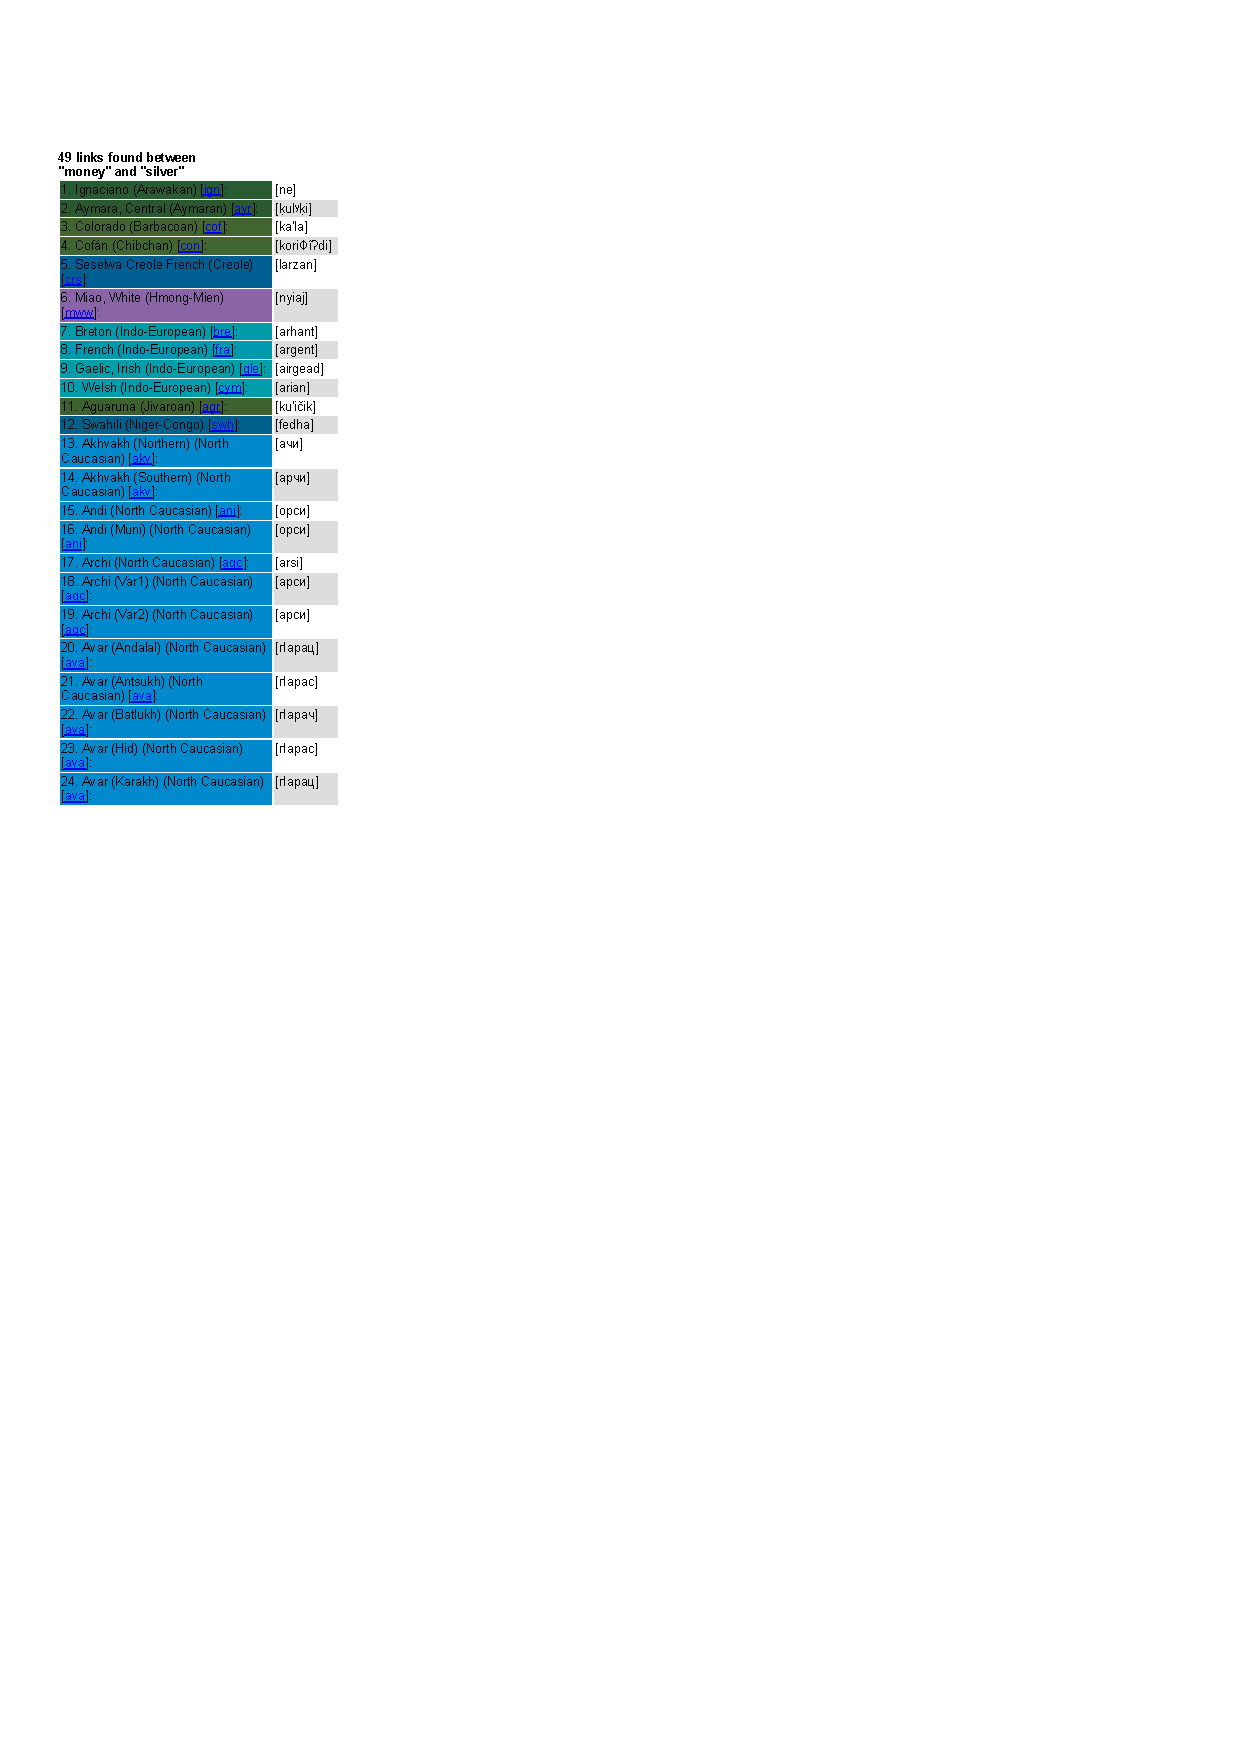
\includegraphics[width=0.238\textwidth]{img/moneysilverAreas1.pdf}
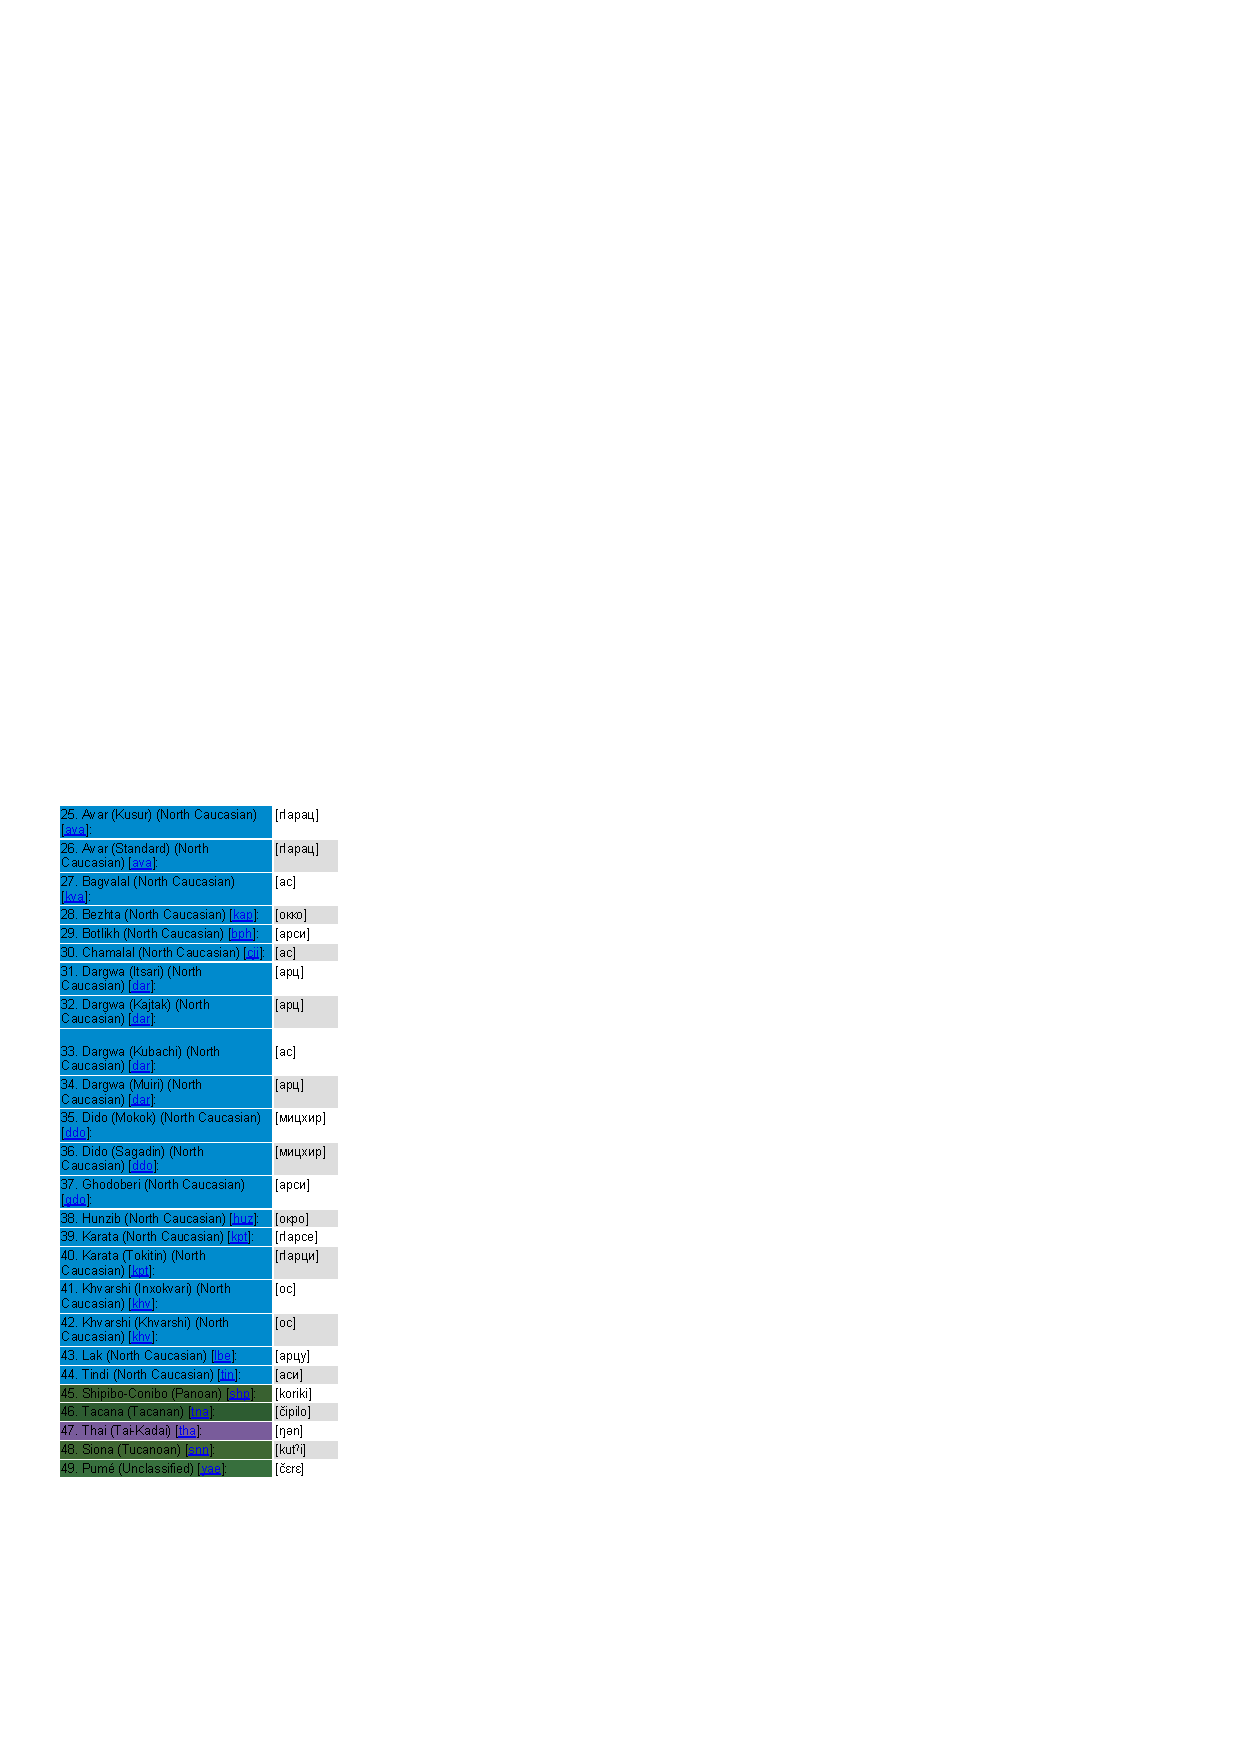
\includegraphics[width=0.238\textwidth]{img/moneysilverAreas2.pdf}
\caption{Languages and words contributing to the connections of lexical associations for the concepts ``money'' and ``silver''}
\label{MoneySilverAreas}
\end{center}
\end{figure}

\begin{figure*}[htbp]
\begin{center}
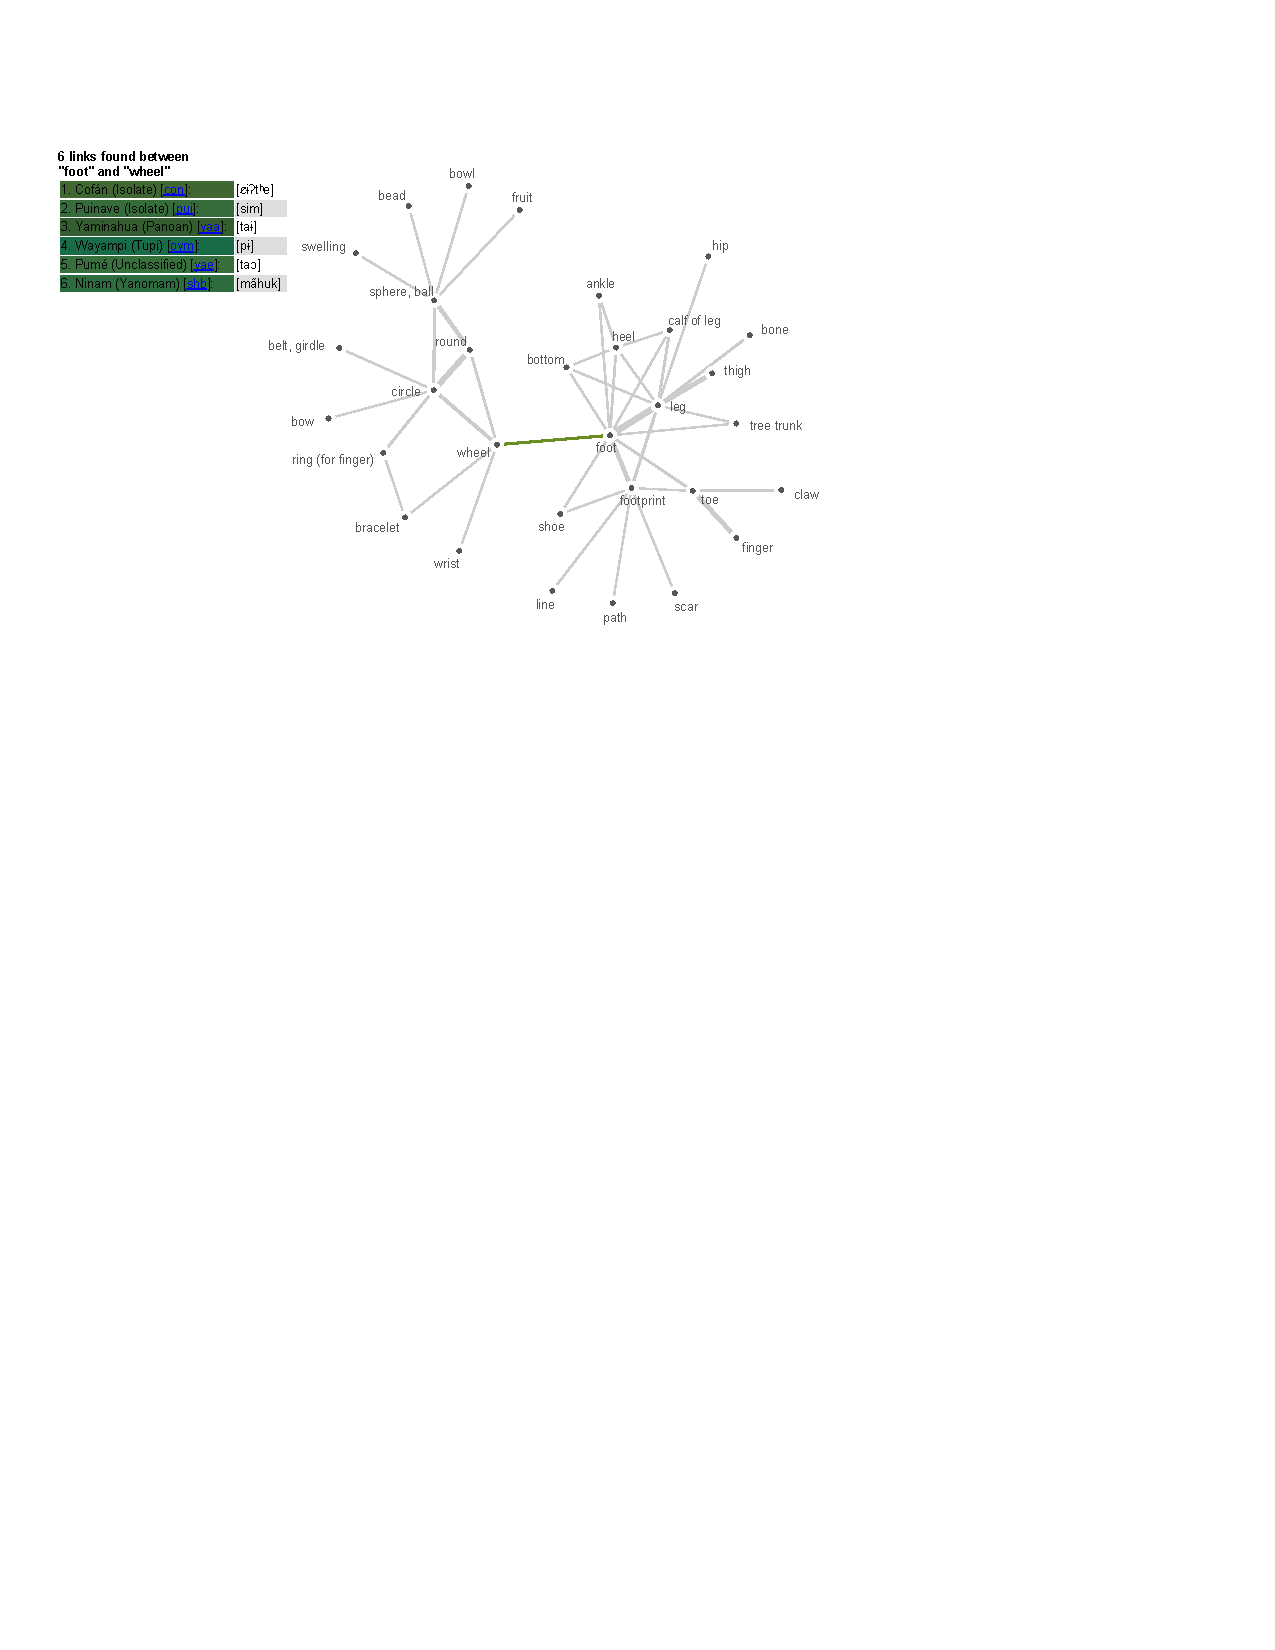
\includegraphics[width=\textwidth]{img/wheelfootAreal.pdf}
\caption{Force-directed graph with areal distribution for the concepts ``wheel'' and ``foot''}
\label{WheelFootAreas}
\end{center}
\end{figure*}


Another example deals with the colexification of the concepts ``wheel'' and ``foot''. In contrast to the case of ``money'' and ``silver'' above, these concepts do not directly suggest a close lexical association. Yet such cases do exits as the link in Figure \ref{WheelFootAreas} reveals. The connection links two bigger communities of nodes, representing spherical objects on the one hand and parts of the lower body on the other. The list of languages for the connection ``wheel'' and ``foot'' in Figure \ref{WheelFootAreas} clearly shows that the association is restricted to languages of South America. Even though the languages cover a range of different families, the areal distribution is clearly confined to a certain area. This might lead to the conclusion that the associations result from loan translations of the concept through language contact (the lexical entries show that they are most likely not cognates and that the association is thus due to loan words for both concepts). However, such a preliminary hypothesis has to be confirmed by looking at the actual data. 



